%%%%%%%%%%%%%%%%%%%%%%%%%%%%%%%%%%%%%%%%%%%%%%%%%%%%%%%%%%%%%%%%%%%%%%
% Reporte del Laboratorio de Metrologia
%%%%%%%%%%%%%%%%%%%%%%%%%%%%%%%%%%%%%%%%%%%%%%%%%%%%%%%%%%%%%%%%%%%%%%
\documentclass[paper=a4, fontsize=11pt]{scrartcl}

\usepackage[T1]{fontenc}
\usepackage{fourier}
\usepackage[spanish]{babel}
\usepackage[protrusion=true,expansion=true]{microtype}
\usepackage{amsmath,amsfonts,amsthm}
\usepackage[pdftex]{graphicx}
\usepackage{url}
\usepackage{booktabs}
\usepackage{float}
\usepackage{caption}

%%% Custom sectioning
\usepackage{sectsty}
\allsectionsfont{\centering \normalfont\scshape}

%%% Custom headers/footers (fancyhdr package)
\usepackage{fancyhdr}
\pagestyle{fancyplain}
\fancyhead{}
\fancyfoot[L]{}
\fancyfoot[C]{}
\fancyfoot[R]{\thepage}
\renewcommand{\headrulewidth}{0pt}
\renewcommand{\footrulewidth}{0pt}
\setlength{\headheight}{13.6pt}

%%% Equation and float numbering
\numberwithin{equation}{section}
\numberwithin{figure}{section}
\numberwithin{table}{section}

%%% Maketitle metadata
\newcommand{\horrule}[1]{\rule{\linewidth}{#1}}

\title{
    \usefont{OT1}{bch}{b}{n}
    \normalfont \normalsize \textsc{Universidad Nacional de Colombia\\
    Sede Bogotá \\
    Facultad de Ingeniería \\
    Departamento de Ingeniería de Sistemas e Industrial \\
    Materia [2026-II]: Tecnología Digital (2016788)
    } \\ [25pt]
    \horrule{0.5pt} \\[0.4cm]
    \huge Reporte del Laboratorio de Metrología \\
    \horrule{2pt} \\[0.5cm]
}

\author{
    \begin{minipage}[t]{0.45\textwidth}
        \centering
        \normalfont \normalsize
        \textbf{Carlos Stiven Romero Sicacha}\\[3pt]
        Ingeniería de Sistemas y Computación\\
        Facultad de Ingeniería\\
        Universidad Nacional de Colombia\\
        \texttt{cromerosi@unal.edu.co}
    \end{minipage}
    \hfill
    \begin{minipage}[t]{0.45\textwidth}
        \centering
        \normalfont \normalsize
        \textbf{Lee Angelo Powell Brant}\\[3pt]
        Ingeniería de Sistemas y Computación\\
        Facultad de Ingeniería\\
        Universidad Nacional de Colombia\\
        \texttt{lpowell@unal.edu.co}
    \end{minipage}
}

\date{}
\graphicspath{{../imagenes/}}

%%% Begin document
\begin{document}
\maketitle

\section*{Resumen}
Se determinó el diámetro exterior de LEDs nominalmente de 5 mm utilizando un pie de rey Mitutoyo 530-104BR. A partir de 32 mediciones se obtuvo una media de $\bar{x}=4.815625$ mm y una desviación estándar muestral de $s=0.068906$ mm. El resultado final fue $V=4.8156\pm0.1466$ mm.\footnote{Código fuente y datos disponibles en: \url{https://github.com/cromerosi/Tecnologia-Digital}}

\section{Objetivos}
\begin{itemize}
    \item Medir el diámetro exterior de LEDs de 5 mm con un pie de rey.
    \item Calcular la media y la desviación estándar muestral de todas las lecturas.
    \item Estimar el error aleatorio y la incertidumbre total de la medición.
    \item Analizar la precisión, la exactitud y la repetibilidad del procedimiento.
\end{itemize}

\section{Instrumento y método experimental}
\subsection{Identificación del instrumento}
El instrumento utilizado fue un pie de rey analógico Mitutoyo, modelo 530-104BR. La etiqueta indica que fue fabricado en Brasil en 2008. Tiene una escala principal en milímetros y un nonio con resolución de 0.05 mm.

Se utilizaron las \textbf{mordazas exteriores}, las dos superficies de mayor tamaño ubicadas en la parte frontal del pie de rey. Se colocaron a ambos lados del cuerpo cilíndrico del LED, perpendicularmente a su eje, hasta establecer un contacto suave con el diámetro exterior. La fuerza aplicada fue apenas suficiente para eliminar la holgura.

\begin{figure}[htbp]
\centering
\begin{minipage}[t]{0.31\textwidth}\centering
    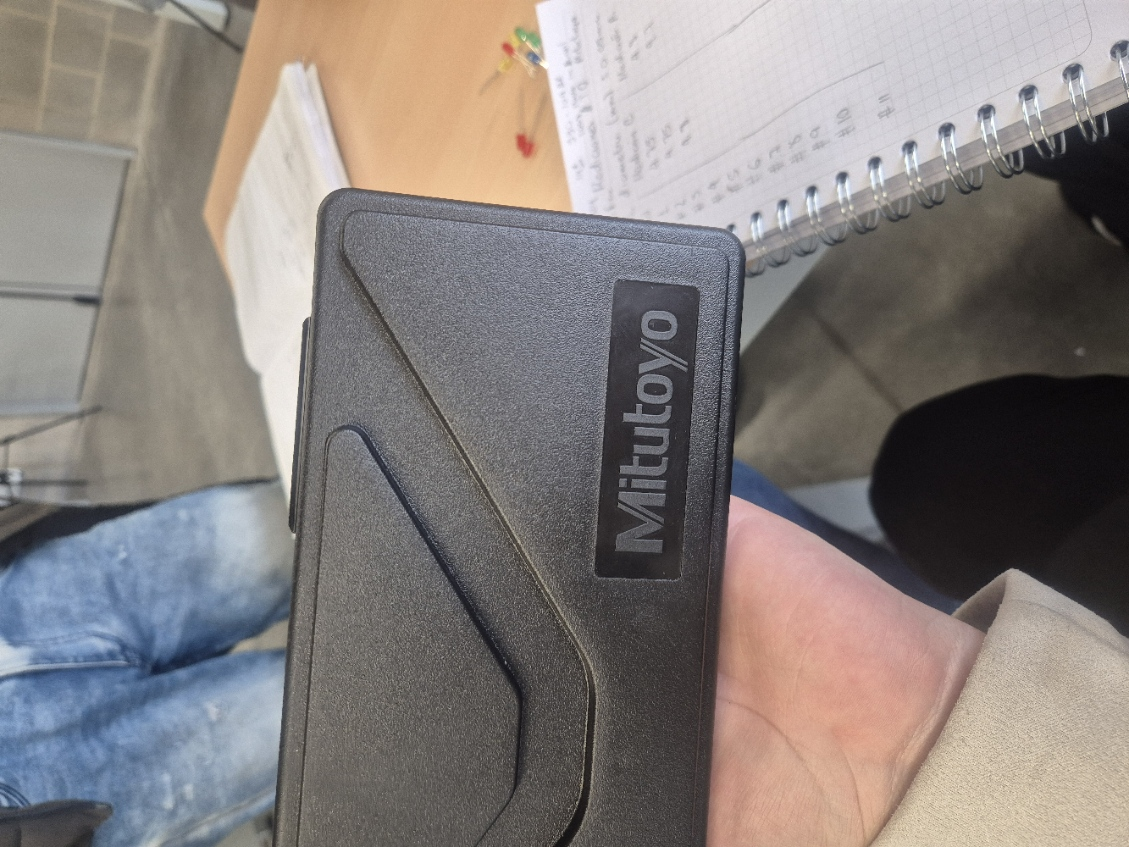
\includegraphics[width=\linewidth]{fig2_caja_mitutoyo.jpg}
    \captionof{figure}{Caja del pie de rey.}
\end{minipage}\hfill
\begin{minipage}[t]{0.31\textwidth}\centering
    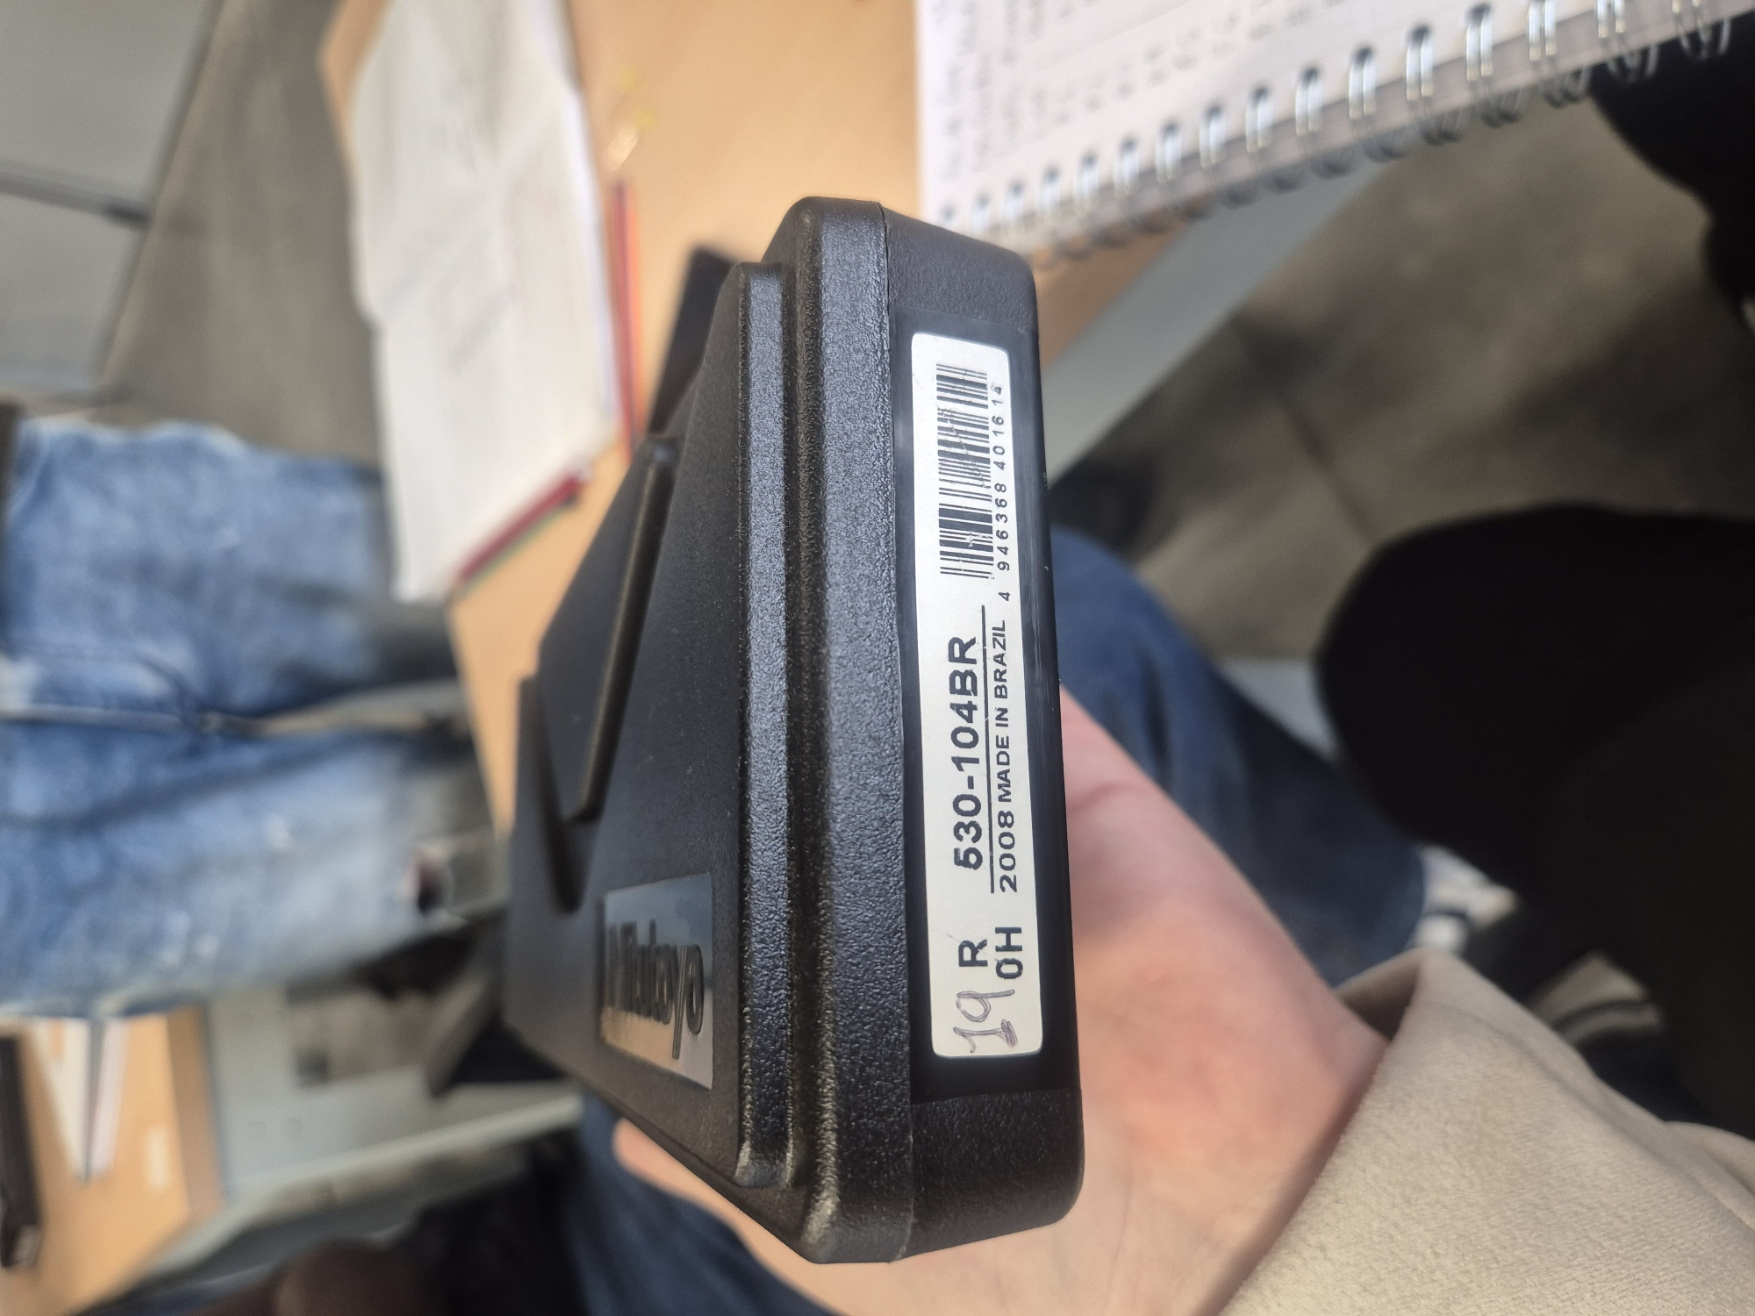
\includegraphics[width=\linewidth]{fig5_estuche_abierto.jpg}
    \captionof{figure}{Pie de rey en su estuche.}
\end{minipage}\hfill
\begin{minipage}[t]{0.31\textwidth}\centering
    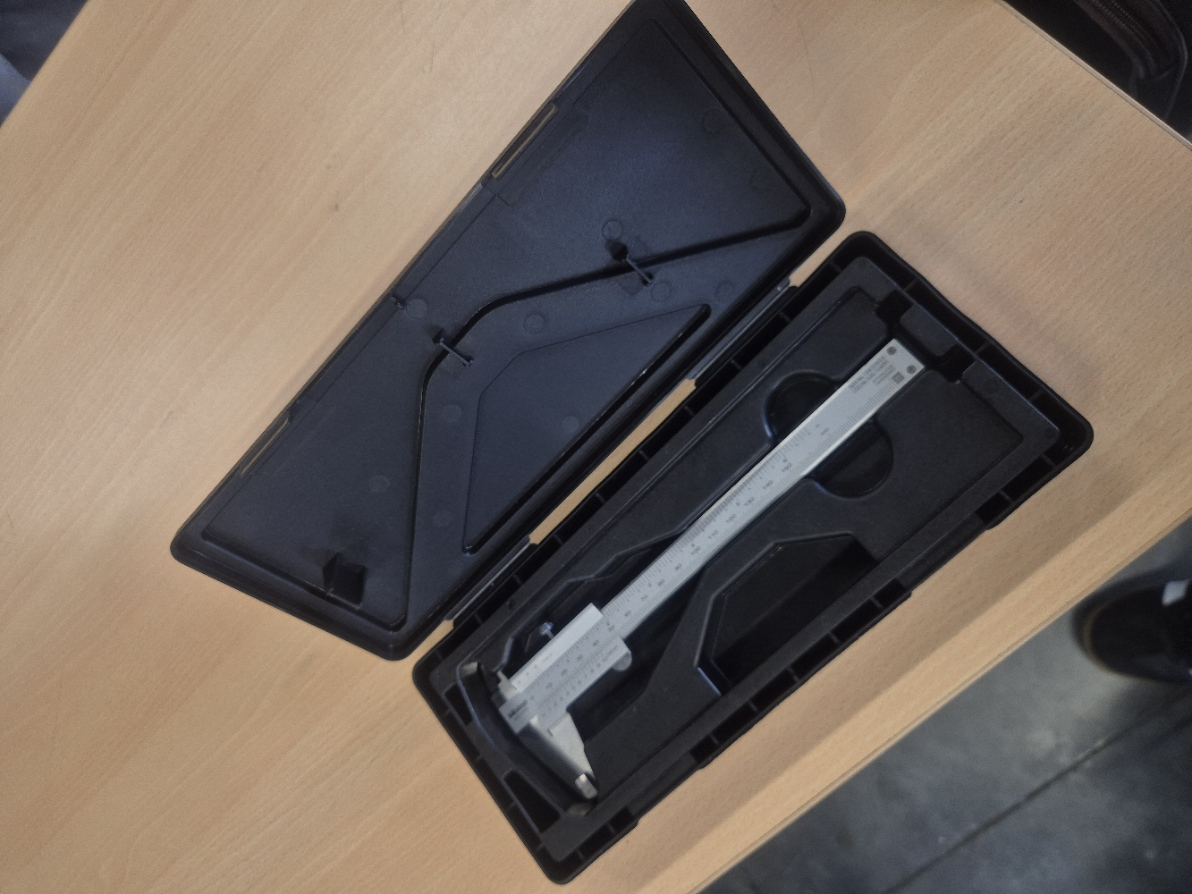
\includegraphics[width=\linewidth]{fig6_serial_mitutoyo_530-104BR.jpg}
    \captionof{figure}{Modelo del instrumento.}
\end{minipage}
\end{figure}

\subsection{Procedimiento}
\begin{enumerate}
    \item Se verificó visualmente el estado del pie de rey y el cierre de sus mordazas.
    \item Se ubicó cada LED transversalmente entre las mordazas exteriores.
    \item Se aplicó una presión ligera y se leyó el valor en milímetros.
    \item Se registraron 32 mediciones en milímetros.
    \item Se calcularon la media y la desviación estándar muestral.
\end{enumerate}

\begin{figure}[htbp]
\centering
\begin{minipage}[t]{0.31\textwidth}\centering
    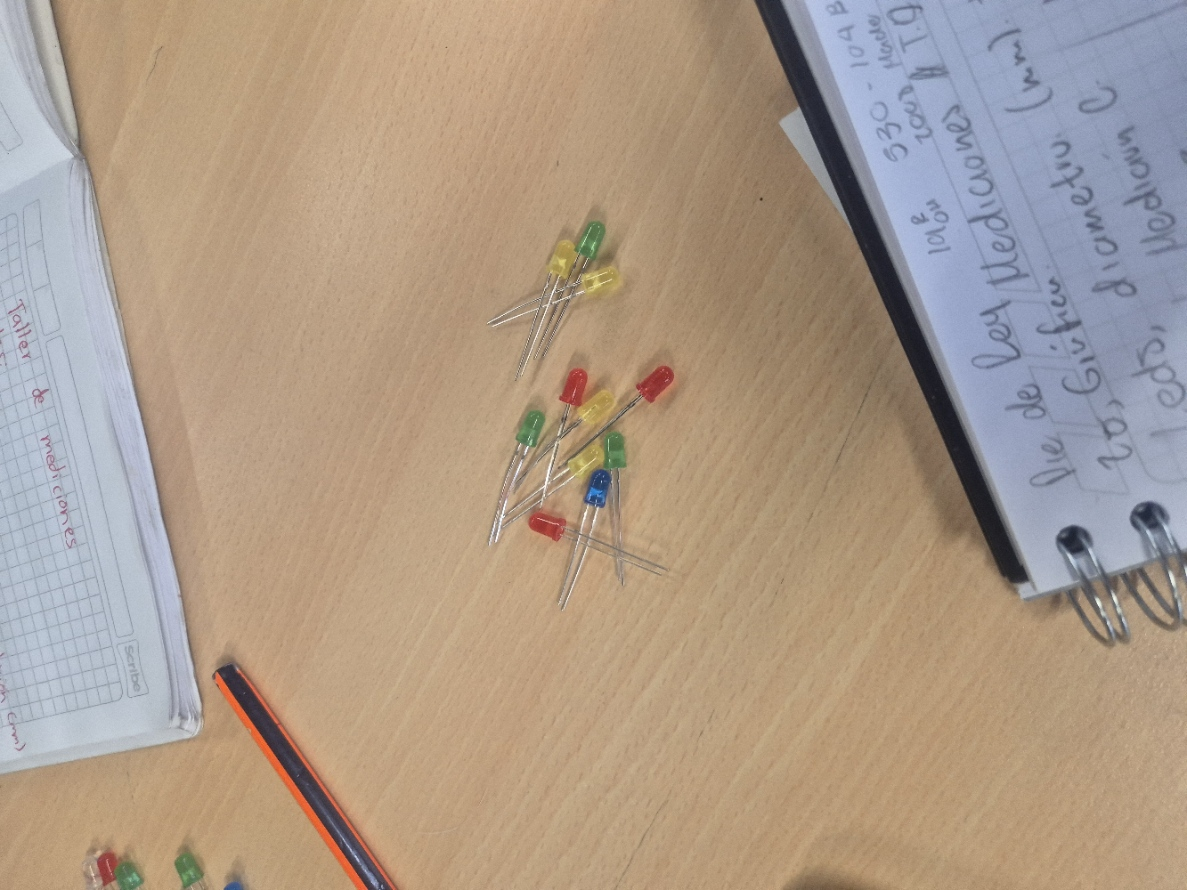
\includegraphics[width=\linewidth]{fig1_leds_lote1.jpg}
    \captionof{figure}{LEDs medidos.}
\end{minipage}\hfill
\begin{minipage}[t]{0.31\textwidth}\centering
    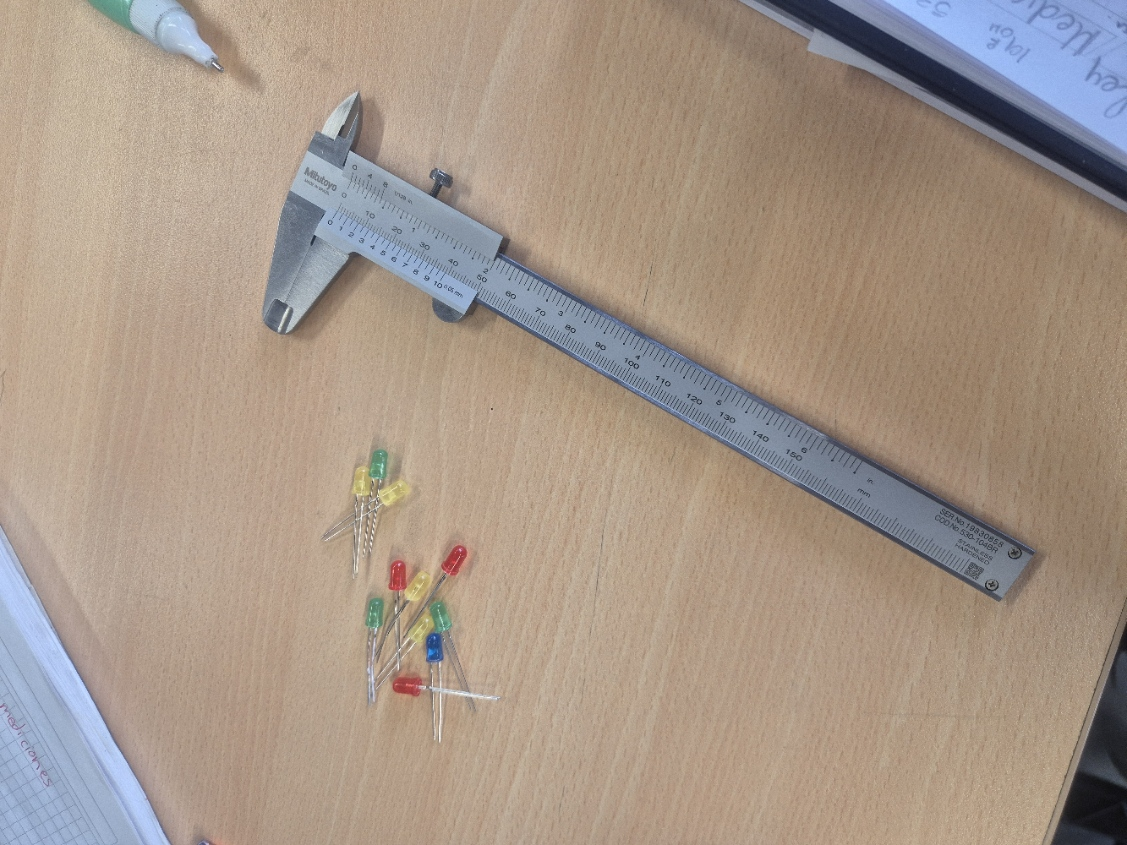
\includegraphics[width=\linewidth]{fig3_led_pie_de_rey.jpg}
    \captionof{figure}{Medición de los LEDs con el pie de rey.}
\end{minipage}\hfill
\begin{minipage}[t]{0.31\textwidth}\centering
    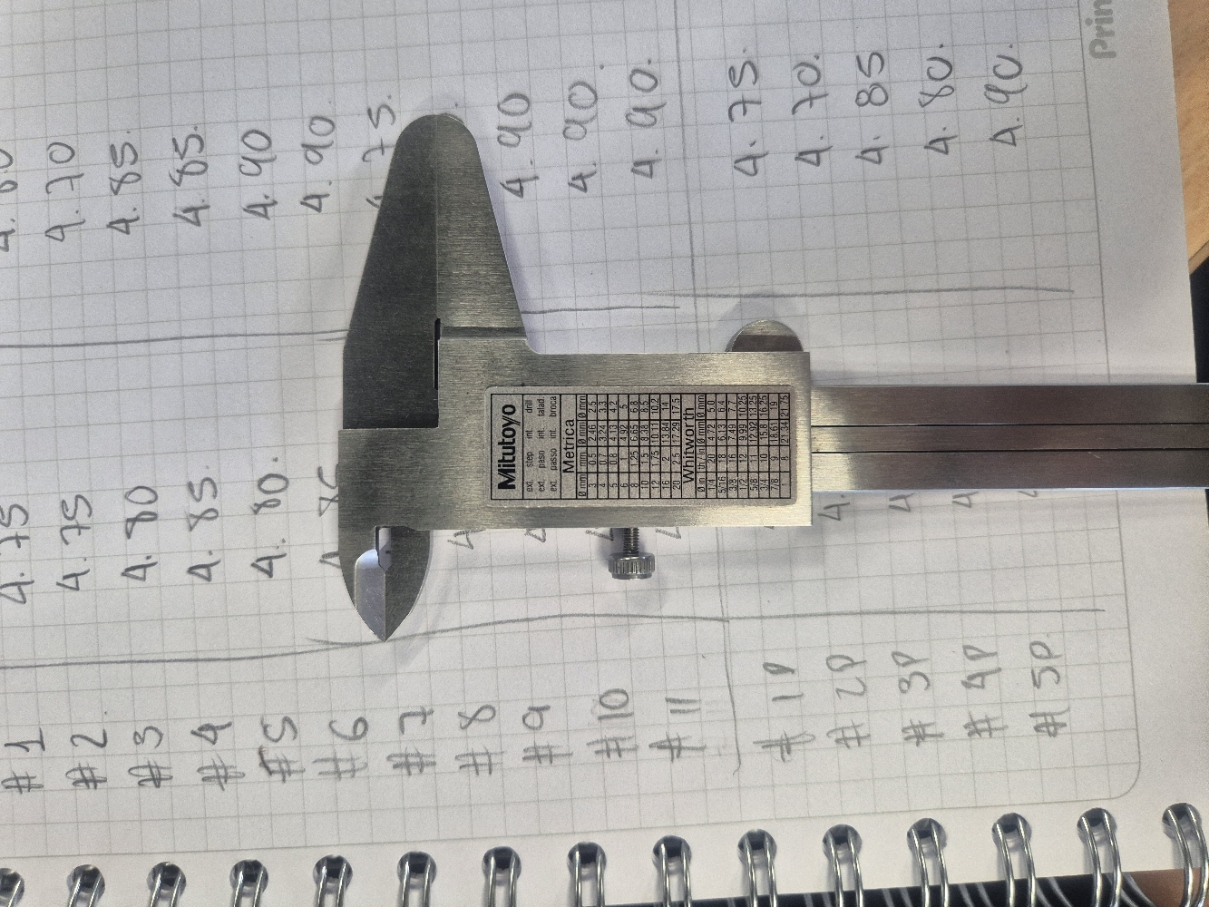
\includegraphics[width=\linewidth]{fig4_mordazas_exteriores.jpg}
    \captionof{figure}{Mordazas exteriores utilizadas para medir el diámetro.}
\end{minipage}
\end{figure}

\section{Datos y análisis estadístico}
Las 32 lecturas se expresaron en milímetros. La suma de las observaciones es $\sum x_i=154.10$ mm. La media y la desviación estándar muestral se calcularon como
\begin{align}
    \bar{x} &= \frac{1}{n}\sum_{i=1}^{n}x_i,\\
    s &= \sqrt{\frac{1}{n-1}\sum_{i=1}^{n}(x_i-\bar{x})^2}.
\end{align}

La media resulta
\begin{equation}
    \bar{x}=\frac{154.10}{32}=4.815625\ \mathrm{mm},
\end{equation}
\noindent y la desviación estándar muestral es
\begin{equation}
    s=0.068906\ \mathrm{mm}.
\end{equation}

Para el nivel aproximado del 95.45\% se definió el error aleatorio como
\begin{equation}
    E_{\mathrm{aleatorio}}=2s=2(0.068906)=0.137811\ \mathrm{mm}.
\end{equation}

Adoptando $U_{\mathrm{inst}}=0.05$ mm, la incertidumbre total se obtiene suponiendo independencia entre la variabilidad observada y el instrumento:
\begin{equation}
    U_{\mathrm{total}}=\sqrt{(2s)^2+U_{\mathrm{inst}}^2}
    =\sqrt{0.137811^2+0.05^2}=0.146601\ \mathrm{mm}.
\end{equation}

Por tanto, el resultado de la medición es
\begin{equation}
    \boxed{V=4.8156\pm0.1466\ \mathrm{mm}}.
\end{equation}

\begin{table}[H]
\centering
\caption{Resumen estadístico de la muestra única.}
\label{tab:estadistica}
\begin{tabular}{lrrrrrr}
\toprule
$n$ & $\sum x_i$ (mm) & $\bar{x}$ (mm) & $s$ (mm) & $2s$ (mm) & $U_{\mathrm{inst}}$ (mm) & $U_{\mathrm{total}}$ (mm)\\
\midrule
32 & 154.1000 & 4.815625 & 0.068906 & 0.137811 & 0.050000 & 0.146601\\
\bottomrule
\end{tabular}
\end{table}

\section{Distribución normal}
La curva representa la distribución normal estimada con $\bar{x}$ y $s$. Cada cruz corresponde a una medición; cuando varias lecturas tienen el mismo valor, las cruces se apilan para mostrar su frecuencia. También se marcan la media y los límites $\bar{x}\pm2s$.

\begin{figure}[htbp]
    \centering
    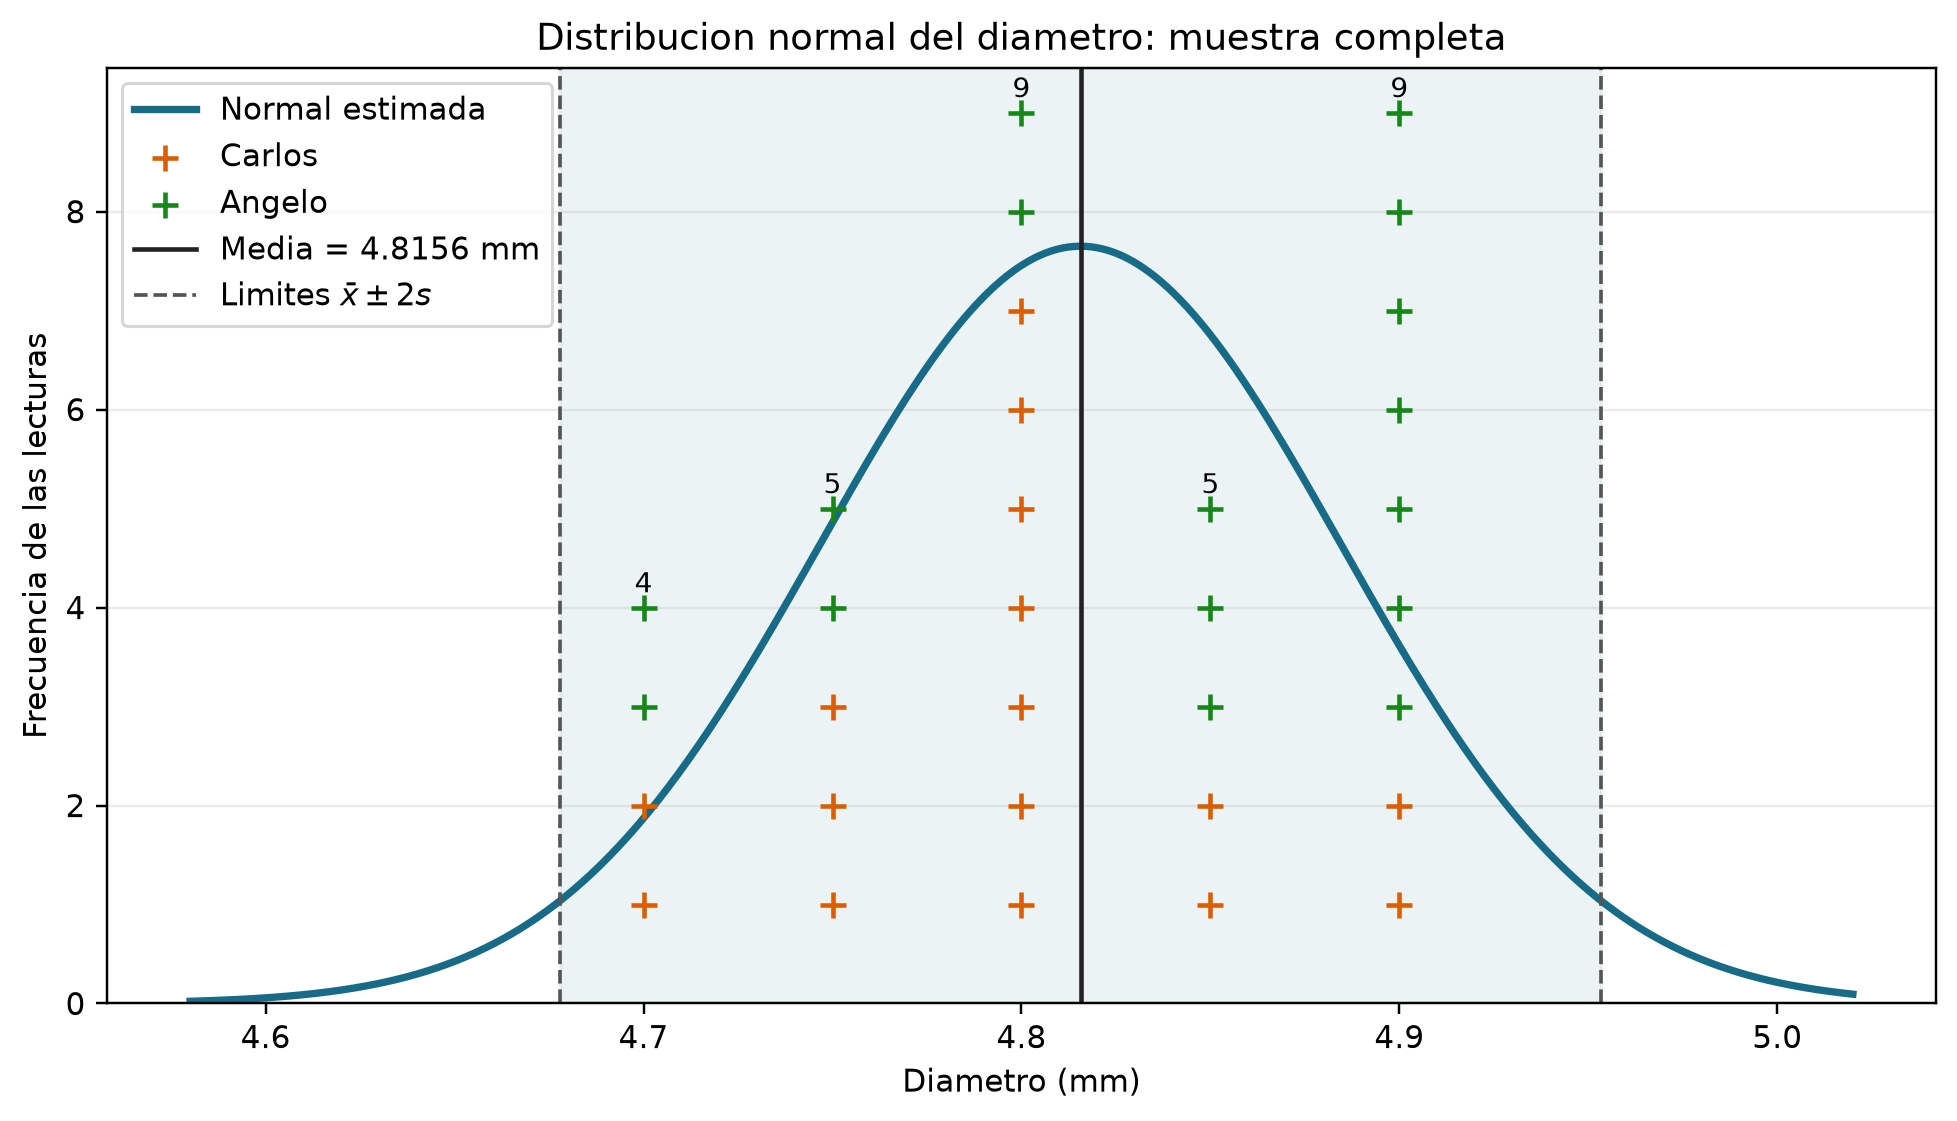
\includegraphics[width=0.88\textwidth]{distribuciones_muestra.png}
    \caption{Distribución normal estimada y lecturas individuales de la muestra completa.}
    \label{fig:distribucion}
\end{figure}

\section{Discusión}
La dispersión de las lecturas, representada por $s=0.068906$ mm, describe la precisión y repetibilidad del procedimiento. Las mediciones se concentran alrededor de 4.82 mm, con pequeñas variaciones debidas al posicionamiento del LED, la fuerza aplicada y la lectura del nonio.

La exactitud no puede establecerse por completo únicamente con estos datos. Para evaluarla sería necesario comparar el resultado con un patrón calibrado o con un valor de referencia trazable. El valor nominal de 5 mm es una referencia comercial del componente, pero no demuestra por sí mismo que la media medida sea exacta.

La contribución aleatoria $2s=0.137811$ mm es mayor que la contribución instrumental de 0.05 mm. Una mejor orientación del LED, una fuerza constante y un mayor número de observaciones ayudarían a reducir la dispersión.

La distribución de las lecturas se concentra en los valores de 4.80 mm y 4.90 mm, con nueve mediciones en cada uno. También se obtuvieron cinco lecturas de 4.75 mm, cinco de 4.85 mm y cuatro de 4.70 mm. Esta agrupación muestra que el instrumento permitió repetir las lecturas en incrementos de 0.05 mm, de acuerdo con la resolución del pie de rey.

La media de 4.815625 mm se encuentra cerca del valor nominal de 5 mm, con una diferencia de aproximadamente 0.184375 mm. Esta diferencia no debe interpretarse solamente como un error del instrumento, ya que también puede incluir variaciones reales entre los LEDs y pequeñas diferencias en la forma de apoyarlos entre las mordazas. El encapsulado plástico tampoco garantiza que todos los componentes tengan exactamente el mismo diámetro.

El resultado representa, por tanto, el comportamiento general de las piezas medidas bajo las condiciones de la práctica. La repetición de valores en la gráfica permite observar la frecuencia de cada lectura y facilita identificar la zona donde se concentra el conjunto de datos. En futuras mediciones sería útil marcar cada LED para seguirlo individualmente y repetir varias veces la medición de una misma pieza. Así se podría distinguir mejor la variación propia de los componentes de la variación causada por el procedimiento.

En términos prácticos, el pie de rey fue adecuado para comprobar que los LEDs corresponden aproximadamente a la dimensión nominal de 5 mm. Sin embargo, el resultado obtenido no debe expresarse con más cifras de las que permite la lectura del instrumento. Los decimales adicionales incluidos en los cálculos sirven para conservar precisión durante las operaciones estadísticas, mientras que el valor reportado con su incertidumbre es el que debe utilizarse para presentar la medición.

\section{Conclusiones}
\begin{enumerate}
    \item Se analizaron 32 mediciones de diámetro exterior.
    \item La media obtenida fue $\bar{x}=4.815625$ mm y la desviación estándar muestral fue $s=0.068906$ mm.
    \item El error aleatorio estimado mediante $2s$ fue $0.137811$ mm.
    \item Con $U_{\mathrm{inst}}=0.05$ mm, la incertidumbre total fue $0.146601$ mm y el resultado final fue $4.8156\pm0.1466$ mm.
    \item La precisión y la repetibilidad se consideran moderadas según la dispersión observada. La exactitud absoluta requiere un patrón de referencia trazable.
\end{enumerate}

El valor obtenido es coherente con el tamaño esperado para este tipo de componente y permite describir de forma sencilla el conjunto de LEDs medidos. La diferencia entre las lecturas más bajas y más altas fue de 0.20 mm, mientras que la mayor parte de los datos quedó agrupada entre 4.75 mm y 4.90 mm. Esto muestra que el resultado no depende de una sola lectura, sino del comportamiento general de la muestra.

Como mejora para una próxima práctica, sería conveniente mantener una orientación idéntica del LED en cada lectura y registrar por separado la pieza medida y la persona que realiza la medición. También se podría comparar el pie de rey con un micrómetro o con un patrón conocido. De esta manera se tendría una referencia adicional para evaluar la exactitud y se podría separar con mayor claridad la variación del instrumento de la variación propia de los componentes.


\end{document}
